


\begin{enumerate}
\item[a)] We use the least squares-estimator introduced in the lecture:
\lz
$\hat{\beta} = (X^TX)^{-1}X^Ty$  with \\ $ X = \begin{bmatrix}
1 & x_{1,1} & x_{1,2} & ... & x_{1,m} \\
2 & x_{2,1} & x_{2,2} & ... & x_{2,m} \\
\vdots & \vdots & \vdots & ... & \vdots \\
n & x_{n,1} & x_{n,2} & ... & x_{n,m} \\
\end{bmatrix}
\lz
$  \\
$ x =  \begin{bmatrix}
0.56  \\
0.22  \\
1.7  \\
0.63  \\
0.36  \\
1.2  \\
\end{bmatrix}, X =  \begin{bmatrix}
1 & 0.56  \\
1 & 0.22  \\
1 & 1.7  \\
1 & 0.63  \\
1 & 0.36  \\
1 & 1.2  \\
\end{bmatrix}
$
and
 $
y =  \begin{bmatrix}
160  \\
150  \\
175  \\
185  \\
165  \\
170  \\
\end{bmatrix}
$

Then \begin{align*}
\hat{\beta} &= (X^TX)^{-1}X^Ty \\ &= \left(
\begin{bmatrix}
1 & 1 & 1 & ... & 1  \\
x_{1,1} & x_{2,1} & x_{3,1} & ... & x_{n,1} \\
\vdots & \vdots & \vdots & ... & \vdots \\
x_{1,m} & x_{2,m} & x_{3,m} & ... & x_{n,m} \\
\end{bmatrix}
\begin{bmatrix}
1 & x_{1,1} & x_{1,2} & ... & x_{1,m} \\
1 & x_{2,1} & x_{2,2} & ... & x_{2,m} \\
\vdots & \vdots & \vdots & ... & \vdots \\
1 & x_{n,1} & x_{n,2} & ... & x_{n,m} \\
\end{bmatrix} \right)^{-1}\begin{bmatrix}
1 & 1 & 1 & ... 1  \\
x_{1,1} & x_{2,1} & x_{3,1} & ... & x_{n,1} \\
\vdots & \vdots & \vdots & ... & \vdots \\
x_{1,m} & x_{2,m} & x_{3,m} & ... & x_{n,m} \\
\end{bmatrix}
\begin{bmatrix}
160  \\
150  \\
175  \\
185  \\
165  \\
170  \\
\end{bmatrix} \\ &= \left(
\begin{bmatrix}
1 & 1 & 1 & 1 & 1 & 1 \\
0.56 & 0.22 & 1.7 & 0.63 & 0.36 &  1.2   \\
\end{bmatrix}
\begin{bmatrix}
1 & 0.56  \\
1 & 0.22  \\
1 & 1.7  \\
1 & 0.63  \\
1 & 0.36  \\
1 & 1.2  \\
\end{bmatrix} \right)^{-1}
\begin{bmatrix}
1 & 1 & 1 & 1 & 1 & 1 \\
0.56 & 0.22 & 1.7 & 0.63 & 0.36 &  1.2   \\
\end{bmatrix}
\begin{bmatrix}
160  \\
150  \\
175  \\
185  \\
165  \\
170  \\
\end{bmatrix} \\ &=
\begin{bmatrix}
6 & 4.67  \\
4.67 & 5.2185   \\
\end{bmatrix}^{-1}
\begin{bmatrix}
1 & 1 & 1 & 1 & 1 & 1 \\
0.56 & 0.22 & 1.7 & 0.63 & 0.36 &  1.2   \\
\end{bmatrix}
\begin{bmatrix}
160  \\
150  \\
175  \\
185  \\
165  \\
170  \\
\end{bmatrix} \\ &=
 \begin{bmatrix}
0.5491944 & -0.4914703  \\
-0.4914703  & 0.6314394   \\
\end{bmatrix}
\begin{bmatrix}
1 & 1 & 1 & 1 & 1 & 1 \\
0.56 & 0.22 & 1.7 & 0.63 & 0.36 &  1.2   \\
\end{bmatrix}
\begin{bmatrix}
160  \\
150  \\
175  \\
185  \\
165  \\
170  \\
\end{bmatrix} \\
&= \begin{bmatrix}
0.2739710 & 0.4410709 & -0.2863051  & 0.23956809 & 0.3722651 & -0.04056998 \\
-0.1378643 & -0.3525536 & 0.5819766 & -0.09366351 & -0.2641521 & 0.26625693 \\
\end{bmatrix}
\begin{bmatrix}
160  \\
150  \\
175  \\
185  \\
165  \\
170  \\
\end{bmatrix} \\
&= \begin{bmatrix}
158.73954  \\
11.25541  \\
\end{bmatrix}
\end{align*}


Hence the linear model $\hat{y} = \hat{\beta}_0 + \hat{\beta}_1 x = 158.73954 + 11.25541 x$

\begin{knitrout}
\definecolor{shadecolor}{rgb}{0.969, 0.969, 0.969}\color{fgcolor}

{\centering 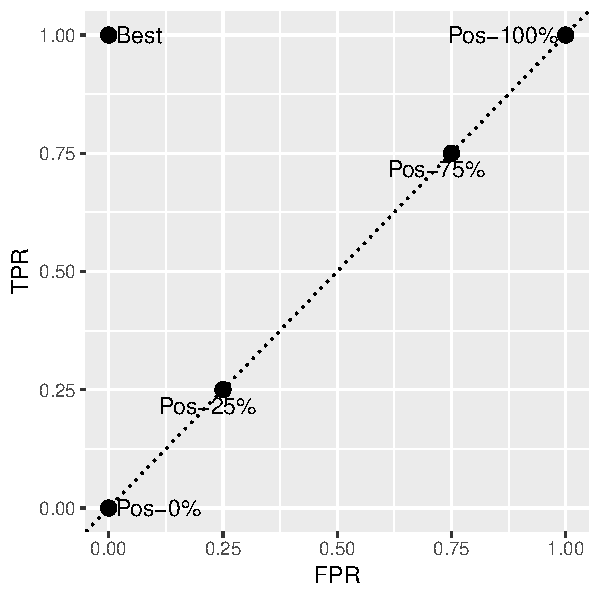
\includegraphics[width=\maxwidth]{figure/unnamed-chunk-2-1} 

}



\end{knitrout}


\item[b)]
Here  $
X =  \begin{bmatrix}
1 & 0.56 & 0.3136 \\
1 & 0.22 & 0.0484 \\
1 & 1.7 & 2.89 \\
1 & 0.63 & 0.3969 \\
1 & 0.36 & 0.1296 \\
1 & 1.2  & 1.44\\
\end{bmatrix}
$
 and $\hat{\beta} =  \begin{bmatrix}
143.51682 \\
57.59155 \\
-23.96347 \\
\end{bmatrix} $


\begin{knitrout}
\definecolor{shadecolor}{rgb}{0.969, 0.969, 0.969}\color{fgcolor}

{\centering 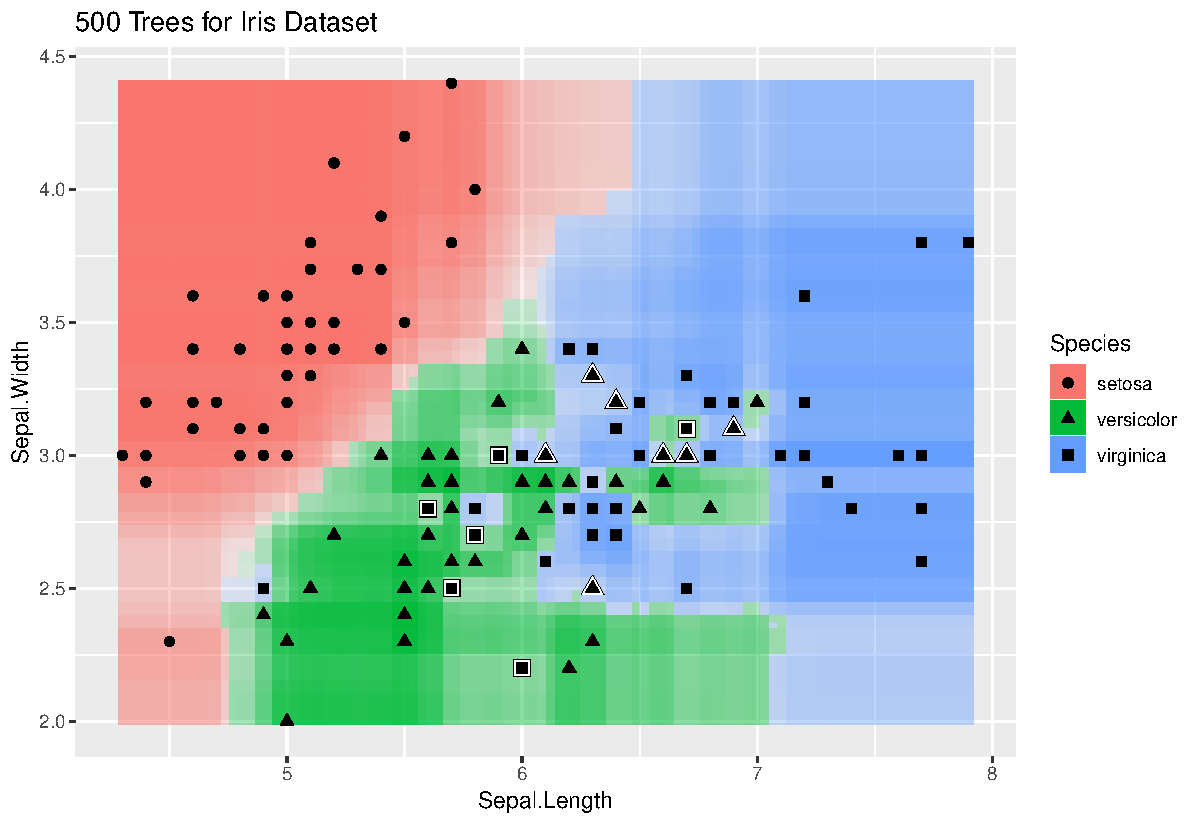
\includegraphics[width=\maxwidth]{figure/unnamed-chunk-3-1} 

}



\end{knitrout}


\end{enumerate}
